
\section[ED para SD]{Estruturas de Dados comuns em P2P}
\subsection{Log Structured Merge Tree}

Agora que você implementou uma DHT totalmente funcional, consideremos os problemas para manipulação dos dados em cada um dos hosts.

\begin{frame}{Large Scale Distributed Databases}
\begin{itemize}
\item Muito dado implica muito IO em disco.
\item Muito IO implica latência elevada.
\pause
\item BD tradicionais usam Árvore B
\item $\log{n}$, para escrita e leitura
\item Lento ou rápido?
\pause 
\item O que é lento em um disco?\pause{} Acessos aleatórios.
\item E se eu não quiser acesso aleatório?
\end{itemize}
\end{frame}

\begin{frame}{Log-Structured Merge Tree}
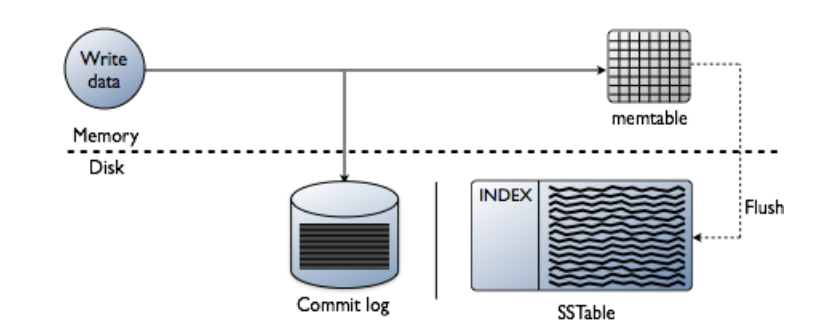
\includegraphics[width=.7\textwidth]{./images/lsm2.png}

\href{https://docs.datastax.com/en/cassandra/3.0/cassandra/dml/dmlHowDataWritten.html}{Fonte}

\begin{itemize}
	\item Durabilidade: Commit log
	\item Limitações de memória: Memória estável
	\item Eficiência de escrita: Escrita sequencial (Log e flush)
	\item Eficiência de leitura: MMDB
	\item Ineficiência de leitura: Múltiplas SSTables
\end{itemize}
\end{frame}

\begin{frame}{Compactação}
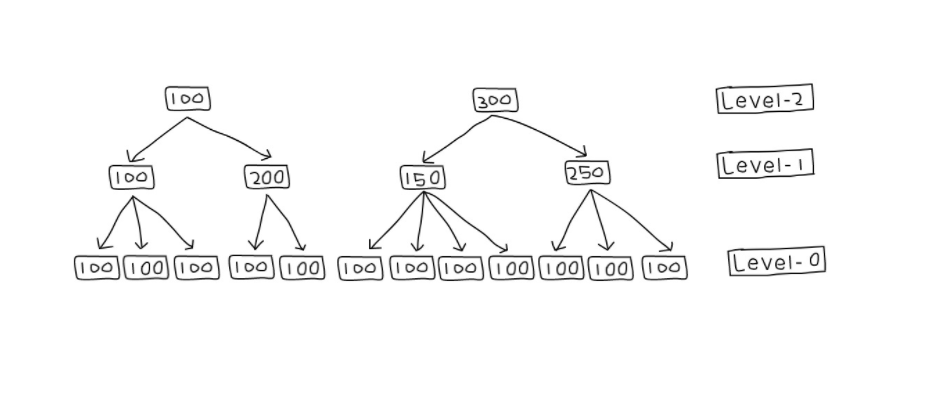
\includegraphics[width=\textwidth]{./images/lsm_compac.png}

\href{https://www.hedvig.io/blog/hedvig-internals-log-structured-merge-trees-and-folding-of-bloom-filters}{Fonte}
\end{frame}



\begin{frame}{Log-Structured Merge Tree}
\begin{itemize}
\item Leitura de disco exige identificar SSTables que possam conter dados
\item Talvez múltiplas sejam necessárias
\item Como identificar rapidamente quais SSTables contém uma chave?
\end{itemize}
\end{frame}




\subsection{Bloom Filter}
\begin{frame}{Bloom-Filter}
\begin{block}{}
	A Bloom filter is a {\color{red}space-efficient} {\color{blue} probabilistic} data structure, conceived by Burton Howard {\color{blue}Bloom} in 1970, that is used to test whether an element is a member of a set. False positive matches are possible, but false negatives are not, thus a Bloom filter has a 100\% recall rate. In other words, a query returns either {\color{blue}``possibly in set''} or {\color{red}``definitely not in set''.}
\end{block}
Sim, é da \href{https://en.wikipedia.org/wiki/Bloom_filter}{Wikipedia}!
\end{frame}


\begin{frame}{LSM + Bloom-Filter}
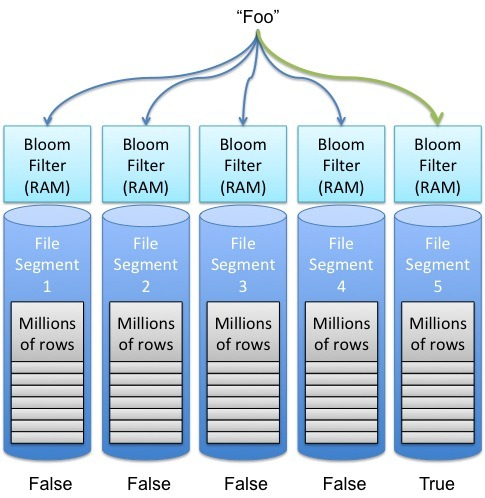
\includegraphics[width=.6\textwidth]{./images/bf_lsm.jpg}

Cada SSTable pode ter índice associado.
\end{frame}

\begin{frame}{Bloom-Filter}
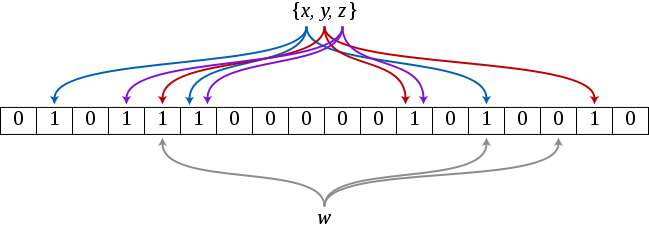
\includegraphics[width=.7\textwidth]{./images/bloom.png}

Na \alert{inserção}, cada elemento passa por várias funcões hash, nesse caso, 3. Cada uma aponta para um índice no filtro, que deve ser virado de 0 para 1.

Na \alert{consulta}, cada elemento passa por pelas mesmas funcões hash. Se algum dos índices apontados não estiver com um 1, o elemento não pertence ao conjunto. Caso contrário, é possível que esteja.

By \href{David Eppstein}{https://commons.wikimedia.org/w/index.php?curid=2609777}
\end{frame}


\begin{frame}{Bloom-Filter}
\begin{itemize}
	\item O número de elementos no conjunto influencia na probabilidade de falsos positivos? \pause Sim!
	\item O número de hashes influencia na probabilidade? \pause Sim!
	\item O número de bits influencia na probabilidade? \pause Sim!
\end{itemize}
\end{frame}

\begin{frame}{Bloom-Filter}
\begin{itemize}
	\item $m$ é o número de bits\\
	A prob. de setar um bit na inserção de um elemento é $1/m$\\
	A prob. de não setar bit é $1 - 1/m$
	
	\item $k$ é número de hashes\\
	A prob. de $k$ hashes não setarem um bit é $(1 - 1/m)^k$
	
	\item $n$ é o número de elementos no filtro\\
	A prob. de não setar um bit após $n$ inserções é $(1 - 1/m)^{kn}$

	\item A prob. de setar um bit $1 - (1 - 1/m)^{kn}$
\end{itemize}

Logo
\begin{itemize}
	\item A prob. de positivo $p = (1 - (1 - 1/m)^{kn})^k \approx (1 - e^{-kn/m})^k$
	\item $m/n = - 1.44\log_2 p$ --- $m$ depende de $n$ e $p$
	\item $k = - \frac{\ln p}{\ln 2} = - \log_2 p$ --- $k$ depende de $p$
\end{itemize}
\end{frame}

\begin{frame}{Bloom-Filter}
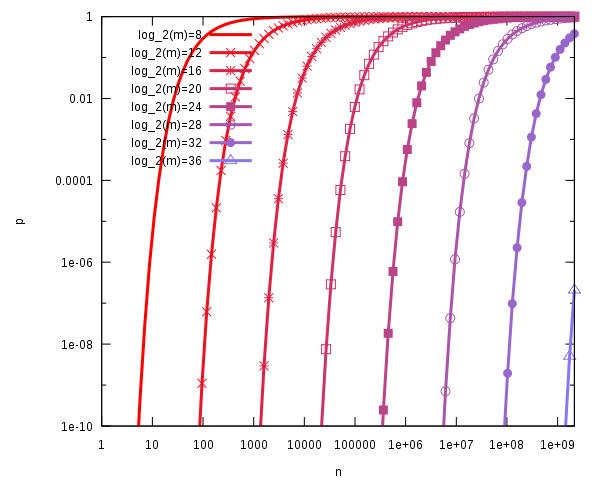
\includegraphics[width=.7\textwidth]{./images/bf_prob.png}

$p$ (eixo $y$) em função de $n$ (eixo $x$) e $m$ (curvas), com $k$ ótimo.

E.g., $m = 2^{24}b = 2MB$ Após 1M inserções, $p = 0,0001$.

By \href{Jerz4835}{https://commons.wikimedia.org/w/index.php?curid=3698803}
\end{frame}


\begin{frame}{Bloom-Filter}
\url{http://www.slideshare.net/quipo/modern-algorithms-and-data-structures-1-bloom-filters-merkle-trees}
\end{frame}


\subsection{Merkle Trees}
\begin{frame}{Como sincronizar duas máquinas?}
Suponha que um mesmo arquivo exista em duas máquinas. Como sincronizá-los de forma eficiente, onde eficiência se mede em termos de uso da rede?

\begin{itemize}
	\item Copie os arquivos de um servidor para outro
	\item Mantenha o mais novo
\end{itemize}

Isso é eficiente?
\end{frame}

\begin{frame}{Como sincronizar duas máquinas?}
\begin{itemize}
		\item Produza um hash dos arquivos
		\item Troque hashes
		\item Se hashes iguais, pronto.
		\item Se hashes diferentes, volte para o slide anterior.
\end{itemize}
\end{frame}

\begin{frame}{Merkle Trees}
	\begin{itemize}
		\item Divida o arquivo em blocos de mesmo tamanho
		\item Faça um hash de cada bloco
		\item Se mais de um hash gerado, 
		\begin{itemize}
			\item Concatene os hashes em um arquivo
			\item Volte para o primeiro item
		\end{itemize}
	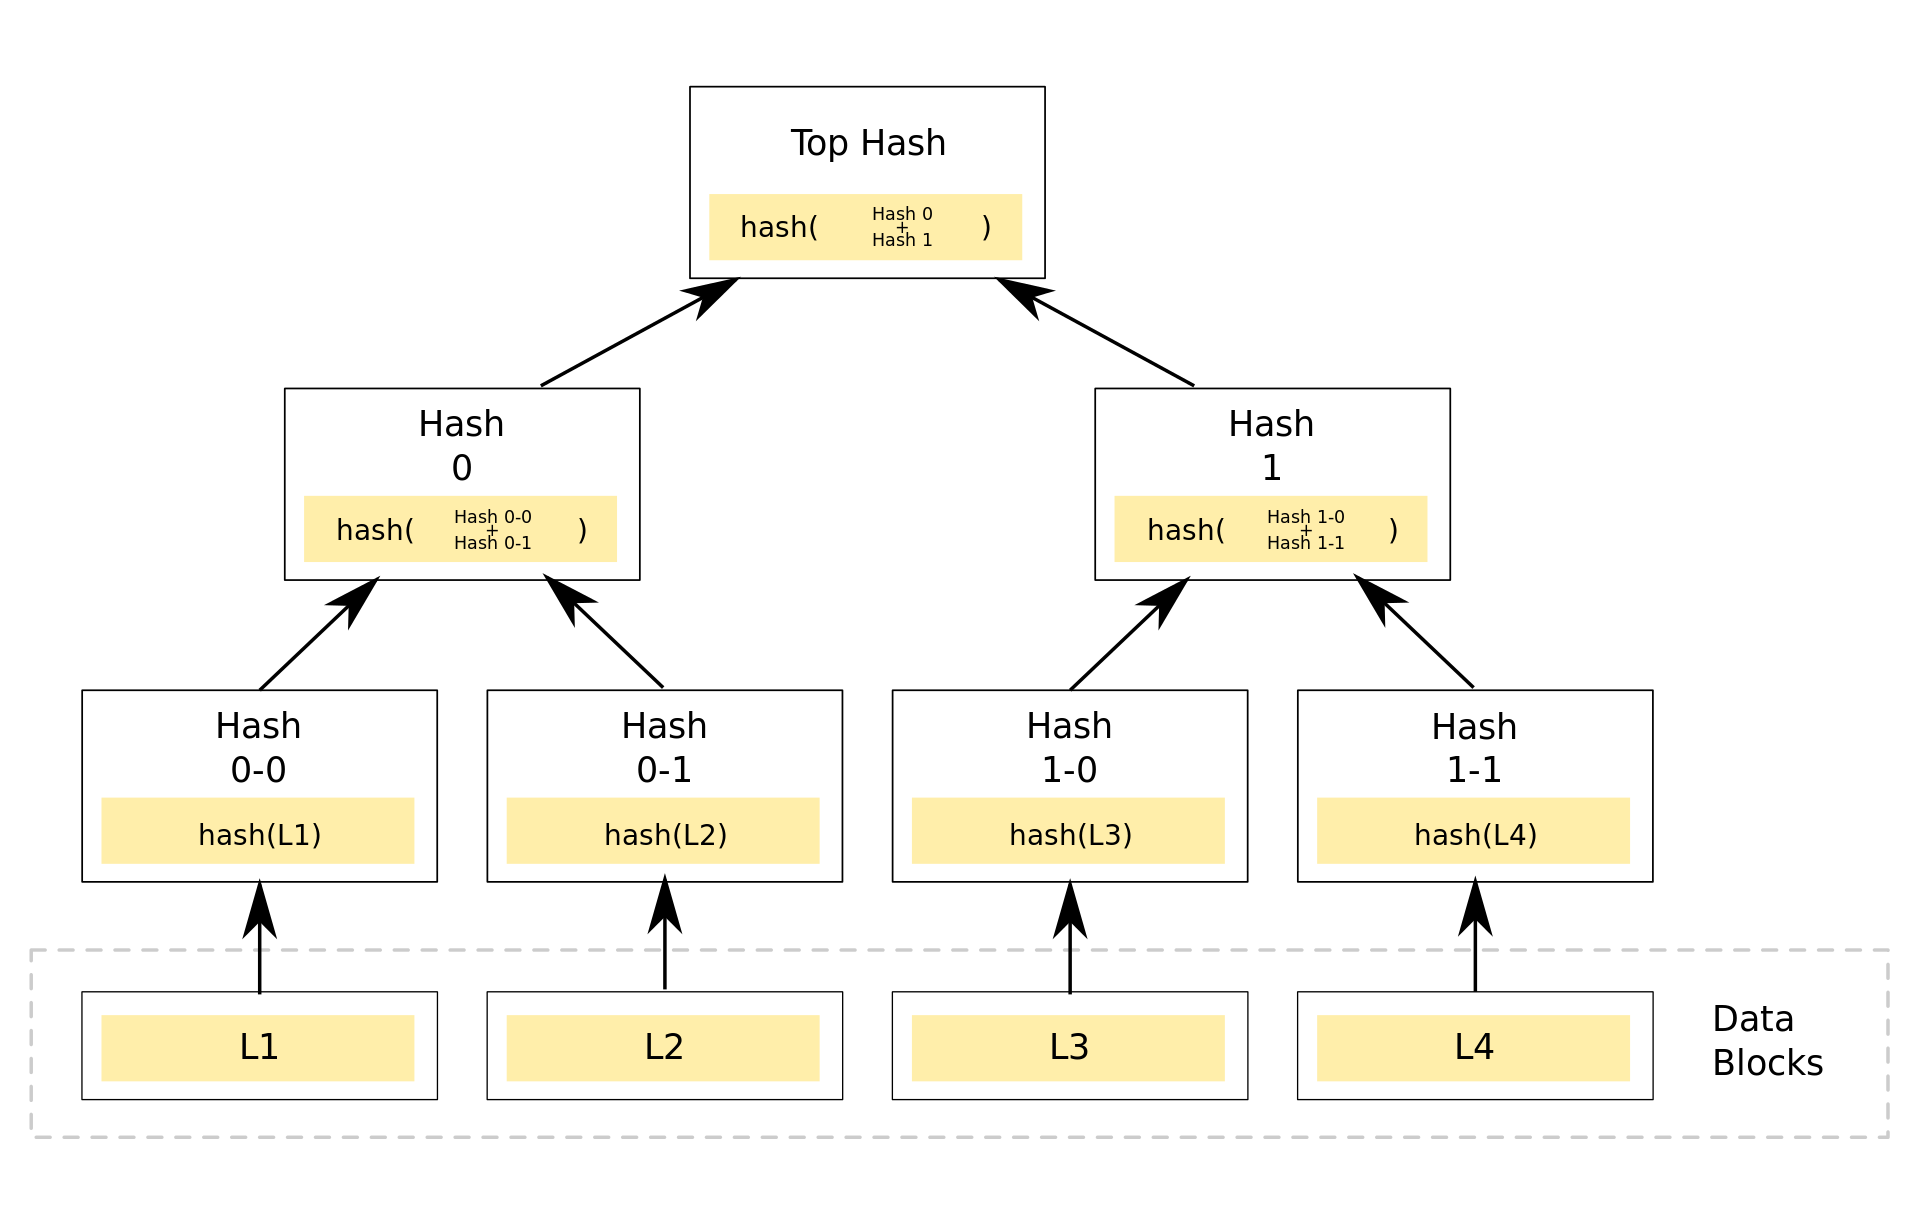
\includegraphics[width=.7\textwidth]{./images/merkle_tree.png} By \href{https://commons.wikimedia.org/w/index.php?curid=18157888}{Azaghal} 
	\end{itemize}
\end{frame}


\begin{frame}{Merkle Trees}
	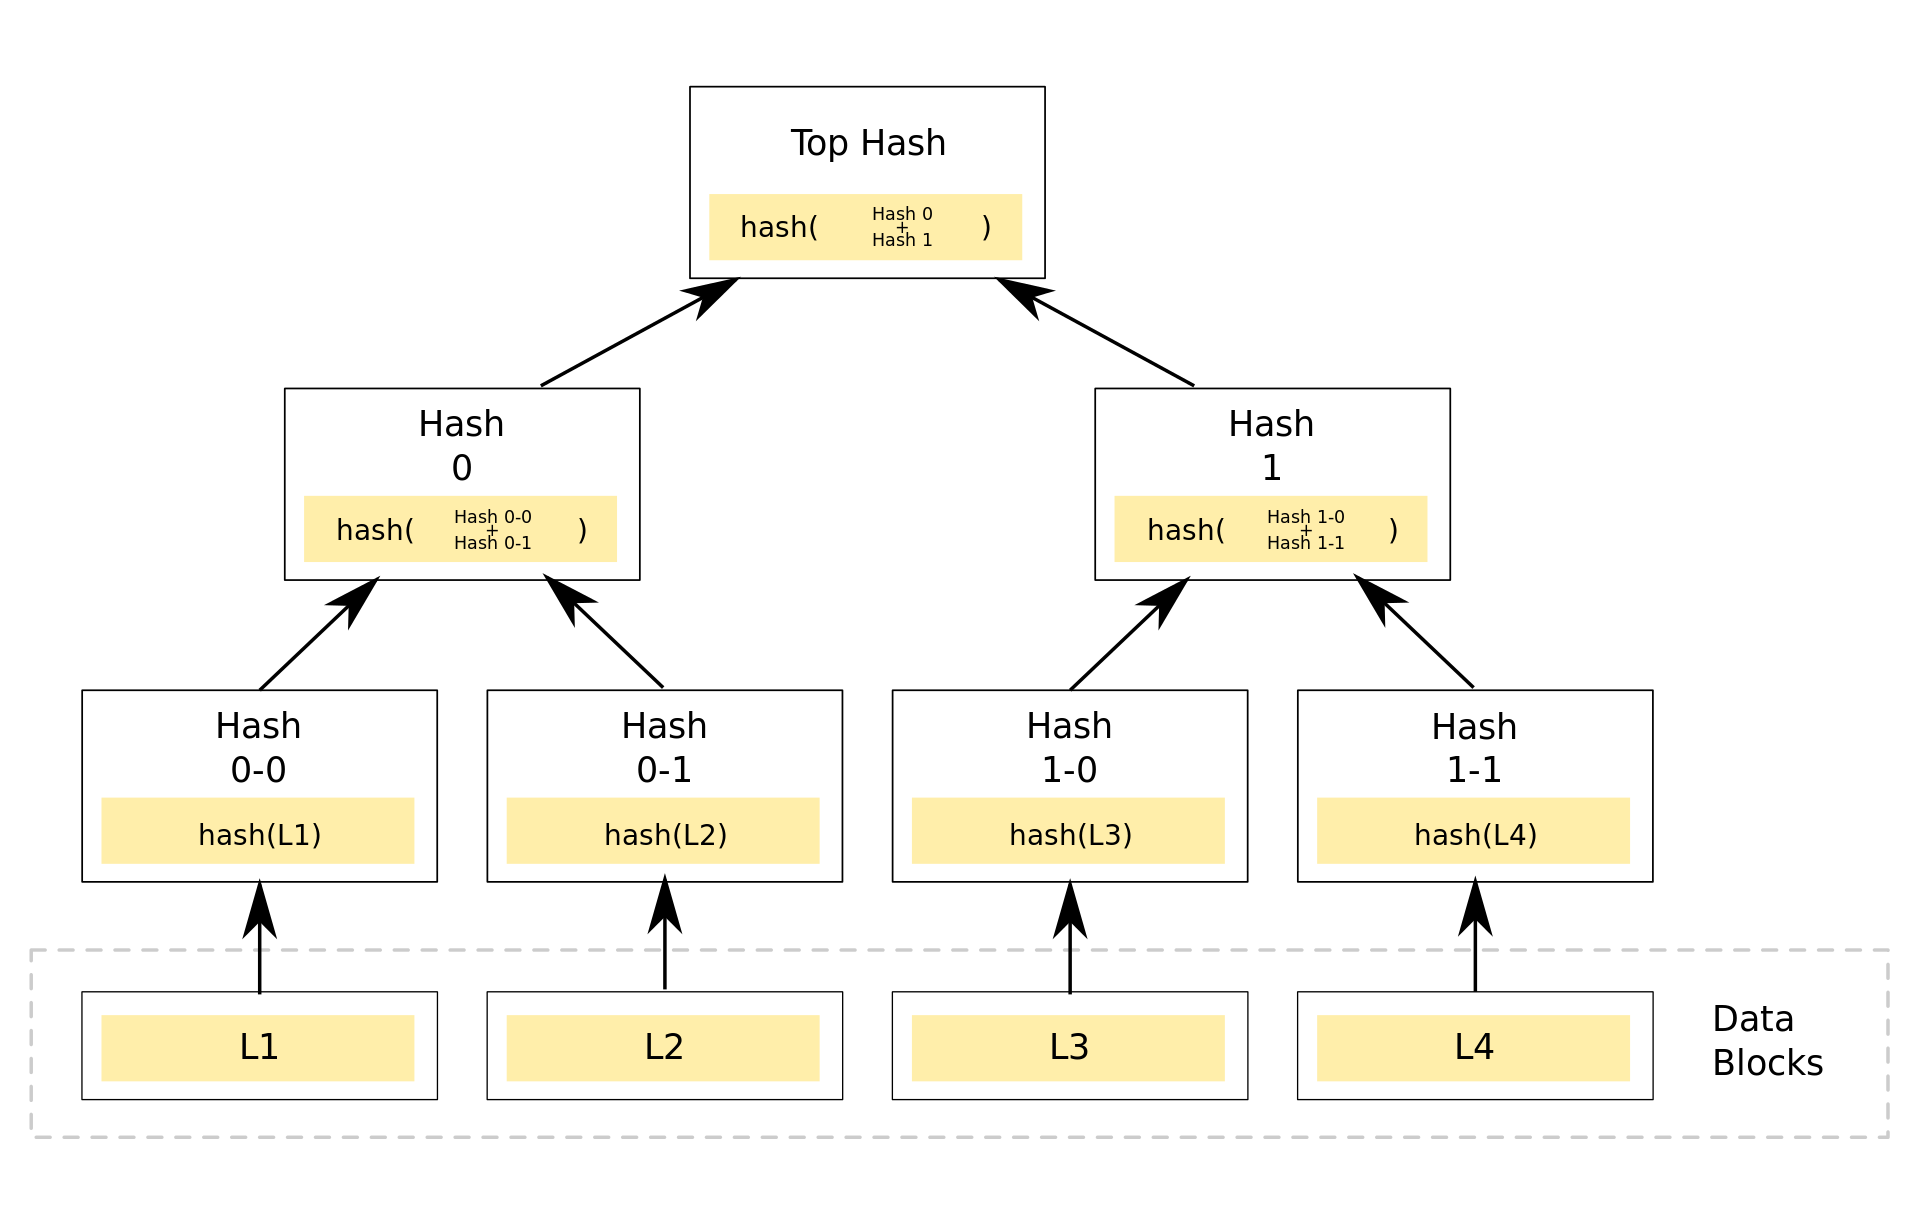
\includegraphics[width=.7\textwidth]{./images/merkle_tree.png} By \href{https://commons.wikimedia.org/w/index.php?curid=18157888}{Azaghal} 

\begin{itemize}
	\item Troque hashes da raiz.
	\item Se hashes iguais, pronto.
	\item Se hashes diferentes \pause compare subárvore.
\end{itemize}
\end{frame}




\begin{frame}{Merkle Trees}
Se a única mudança no arquivo foi a adição de um byte no começo do arquivo?
\end{frame}

\begin{frame}{Merkle-Tree}
\url{http://www.slideshare.net/quipo/modern-algorithms-and-data-structures-1-bloom-filters-merkle-trees}	
\end{frame}


\begin{frame}{Rabin Fingerprint}

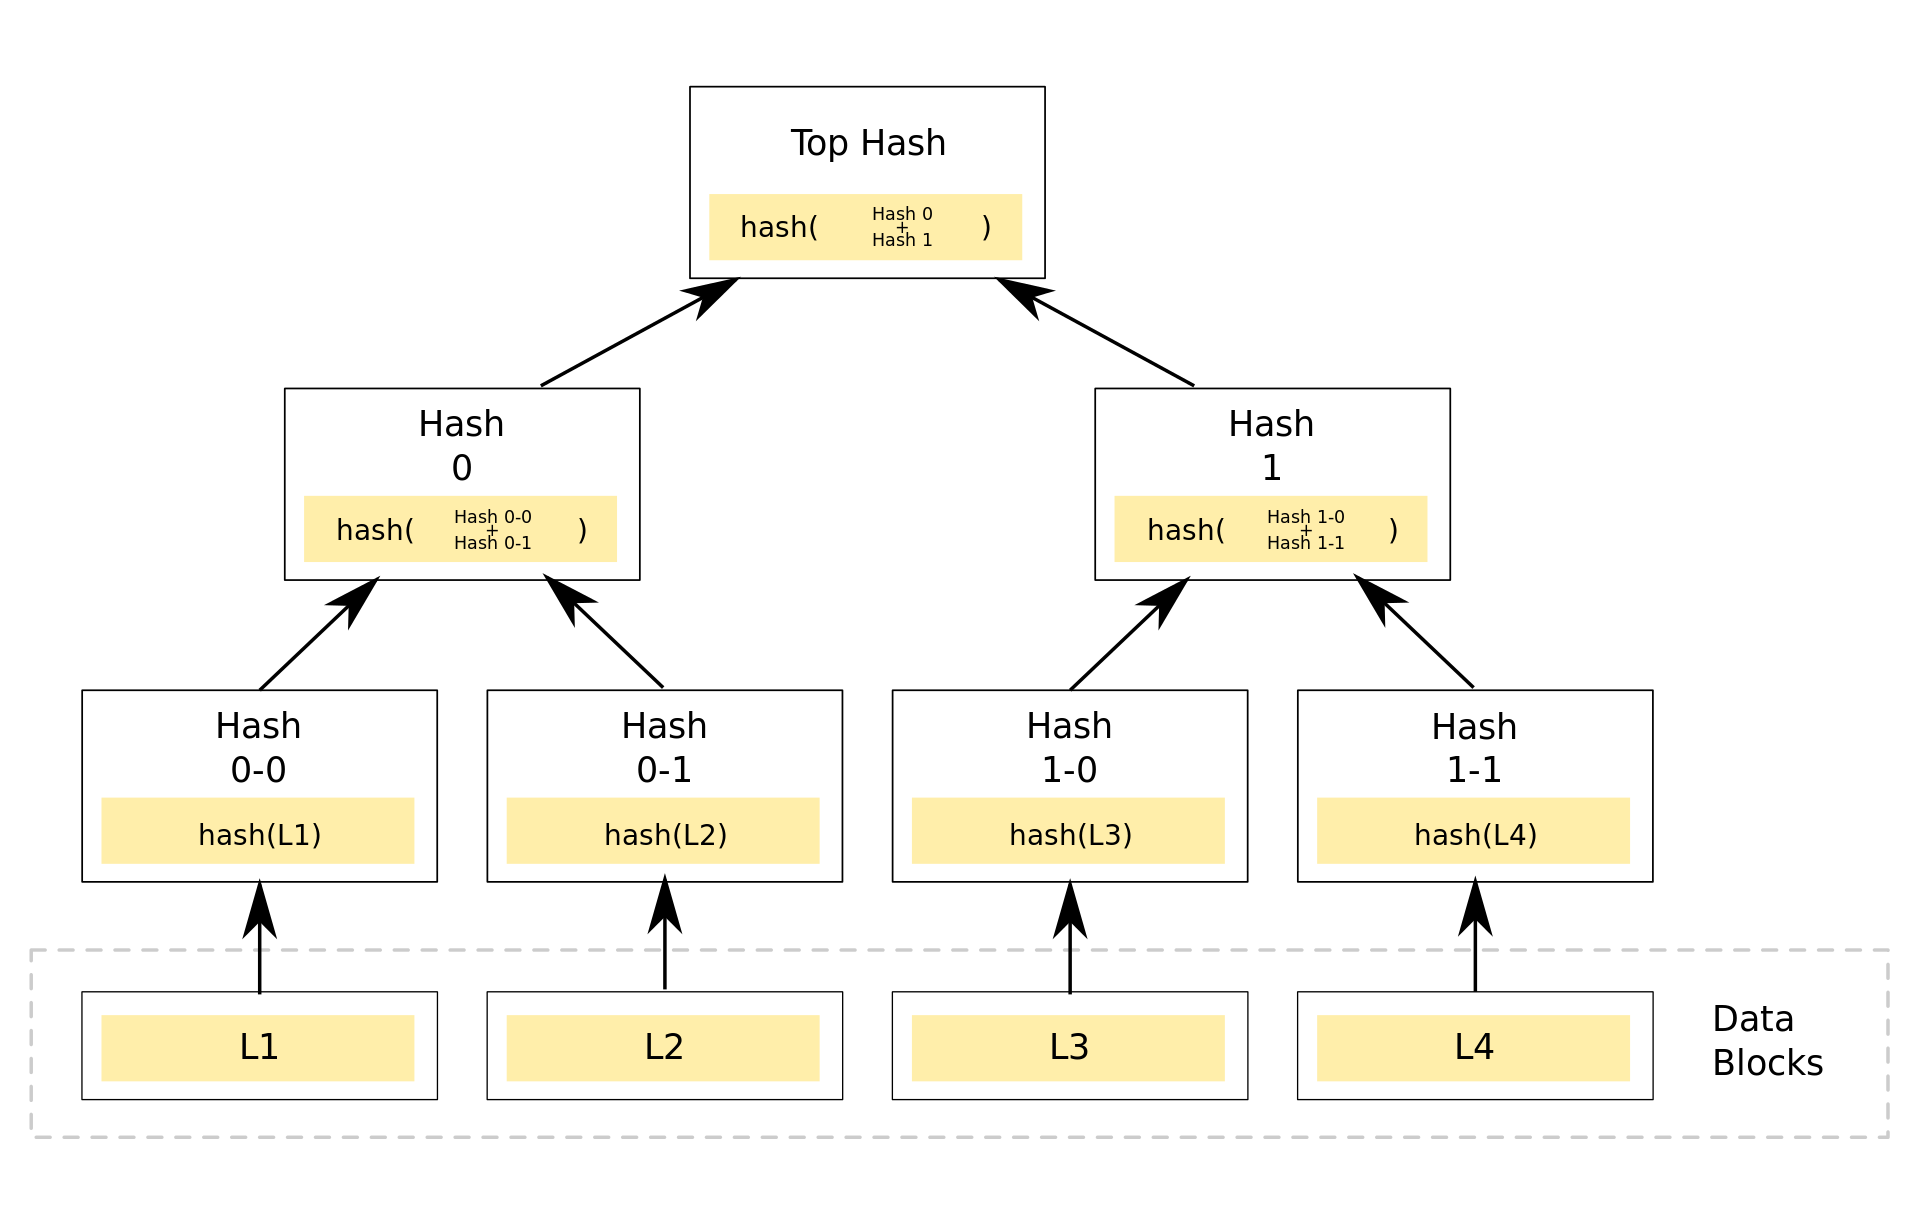
\includegraphics[width=.7\textwidth]{./images/merkle_tree.png}

Fonte \url{https://moinakg.wordpress.com/tag/minhash/} 
\end{frame}


\begin{frame}{Rabin Fingerprint}
	
	
\url{https://en.wikipedia.org/wiki/Rolling_hash}
\end{frame}
